% Provenance (never printed): the markets-with-algebra strand of ../economics_series.md (grade 9: price ceiling and
% floor; a tax per unit and who bears it; a subsidy as a negative tax; each with a documented episode). Brief:
% sources/book1/BRIEFS.md, g9-03. "Tax incidence" and "deadweight loss" are grade 10's: here in words, no definitions.
% Chart data: figdata/grade-9/03-price-controls-taxes-subsidies (published rent-control estimates, each a ledger row;
% the worked example of g9-01; an invented milk market). Ledger: g9:dmq-2019-stay, -supply, -rents;
% g9:fuel-tax-cut-2022. Note: with Q^d = a - bp and Q^s = c + dp, a tax t on sellers raises the buyer's price by
% t d/(b + d) (the brief's "t b/(b+d)" is the seller's share).
\chapter{Price Controls, Taxes and Subsidies}\label{ch:g9:price-controls-taxes-subsidies}

\begin{openingchart}{San Francisco extended rent control in 1994 to more rental buildings, in percent. Two
effects measured by comparing the newly covered buildings with similar buildings that were not covered
(solid bars), and one city-wide rent rise that the authors calculate from those estimates (hatched
bar).}{Diamond, McQuade and Qian (2019)}
\begin{tikzpicture}
\begin{axis}[omrecord, xbar, bar width=12pt, y=0.9cm, xmin=-20, xmax=25, width=0.66\linewidth,
  ytick={0,1,2}, yticklabels from table={figdata/grade-9/03-price-controls-taxes-subsidies/out/rent_control.csv}{effect},
  yticklabel style={font=\footnotesize, align=right, text width=4.2cm}, enlarge y limits={abs=0.6},
  xlabel={Change (percent)}, extra x ticks={0}, extra tick style={grid style={black!60, thin}},
  nodes near coords, nodes near coords style={font=\footnotesize},
  every node near coord/.append style={/pgf/number format/showpos}]
\addplot[fill=omDef, draw=none, bar shift=0pt] table[x=measured, y=pos]
  {figdata/grade-9/03-price-controls-taxes-subsidies/out/rent_control.csv};
\addplot[draw=omDef, pattern=north east lines, pattern color=omDef, bar shift=0pt] table[x=estimated, y=pos]
  {figdata/grade-9/03-price-controls-taxes-subsidies/out/rent_control.csv};
\end{axis}
\end{tikzpicture}
\end{openingchart}

% ledger: g9:dmq-2019-stay, g9:dmq-2019-supply, g9:dmq-2019-rents
A rent control caps the rent that landlords may charge sitting tenants. In San Francisco, when the 1994
rule extended it to more buildings, the tenants of those buildings became nearly $20\,\%$ more likely to
stay at their address: the rule protected them from rent rises. The landlords of the same buildings
reduced the housing they offered for rent by $15\,\%$. The authors then calculate that, with fewer flats
for rent, rents across the city were about $5.1\,\%$ higher. That number is not measured like the
other two: it comes from the $15\,\%$ cut and an assumed response of renters to rents.

Governments often set \omterm{def:g7:money:price}{prices}, or \omterm{def:g8:taxes-and-public-spending:tax}{tax} and subsidise goods, to help some buyers or sellers. The supply and
demand lines of \cref{ch:g9:demand-and-supply-equations} predict what follows, and who gains.

\begin{recall}
At a \omterm{def:g7:money:price}{price} where the \omterm{def:g7:demand-and-supply-first-look:quantity-demanded}{quantity demanded} is larger than the \omterm{def:g7:demand-and-supply-first-look:quantity-supplied}{quantity supplied} there is a \omterm{def:g7:markets-and-prices:shortage}{shortage}; where
it is smaller, a \omterm{def:g7:markets-and-prices:market-surplus}{market surplus} (\cref{ch:g7:markets-and-prices}). With $Q^d = a - b\,p$ and $Q^s = c + d\,p$,
the \omterm{def:g7:demand-and-supply-first-look:equilibrium-price}{equilibrium price} is $(a - c)/(b + d)$ (\cref{ch:g9:demand-and-supply-equations}). The elasticity
measures how much buyers respond to the \omterm{def:g7:money:price}{price} (\cref{ch:g9:elasticity-first-look}).
\end{recall}

All the numbers of this chapter use the worked example of
\cref{ch:g9:demand-and-supply-equations}: demand $Q^d = 120 - 4p$, supply $Q^s = 20 + 6p$, \omterm{def:g7:demand-and-supply-first-look:equilibrium-price}{equilibrium
price} 10 dalens and quantity 80 units.

\section{A maximum price}

\begin{definition}[Price ceiling]\label{def:g9:price-controls-taxes-subsidies:price-ceiling}
A \emph{price ceiling}\index{price ceiling} is a maximum \omterm{def:g7:money:price}{price} set by law: sellers may not charge
more.
\end{definition}

A ceiling of 8 dalens, below the \omterm{def:g7:demand-and-supply-first-look:equilibrium-price}{equilibrium price} of 10, gives a \omterm{def:g7:demand-and-supply-first-look:quantity-demanded}{quantity demanded} of $120 - 32 = 88$
units and a \omterm{def:g7:demand-and-supply-first-look:quantity-supplied}{quantity supplied} of $20 + 48 = 68$. Only 68 units are sold, and 20 units that buyers want at
that \omterm{def:g7:money:price}{price} are not available: a \omterm{def:g7:markets-and-prices:shortage}{shortage} of 20.

\begin{model}{A price ceiling}
\assumes Many buyers and sellers; a legal maximum \omterm{def:g7:money:price}{price} below the \omterm{def:g7:demand-and-supply-first-look:equilibrium-price}{equilibrium price}.
\predicts A \omterm{def:g7:markets-and-prices:shortage}{shortage} equal to $Q^d - Q^s$ at the ceiling; fewer units sold than without the ceiling;
the goods go to whoever comes first, knows the seller or accepts a lower quality; sellers spend less on
upkeep.
\tested Rent control in San Francisco (opening chart): the covered landlords offered $15\,\%$ less housing
for rent.
\breaks A ceiling above the \omterm{def:g7:demand-and-supply-first-look:equilibrium-price}{equilibrium price} has no effect; trading at higher \omterm{def:g7:money:price}{prices} outside the law
(a black \omterm{def:g7:markets-and-prices:market}{market}) reduces the \omterm{def:g7:markets-and-prices:shortage}{shortage} but not the number of units produced.
\end{model}

\begin{omfigure}
\begin{tikzpicture}[econ, x=0.042cm, y=0.32cm]
  \draw[econ axes] (0,21) node[above, font=\scriptsize] {price} |- (165,0) node[right, font=\scriptsize] {quantity};
  \draw[demand] (40,20) -- (120,0) node[pos=0.08, right, font=\scriptsize] {demand};
  \draw[supply] (20,0) -- (140,20) node[pos=0.95, left, font=\scriptsize] {supply};
  \draw[thick, black] (0,8) -- (150,8) node[right, font=\scriptsize] {ceiling};
  \node[eqpoint, fill=black!45] at (80,10) {};
  \draw[guide] (68,8) -- (68,0) node[below, font=\scriptsize] {68};
  \draw[guide] (88,8) -- (88,0) node[below, font=\scriptsize] {88};
  \draw[<->, thick] (68,1.5) -- (88,1.5) node[right, font=\scriptsize] {shortage};
  \node[left, font=\scriptsize] at (0,8) {8};
  \node[left, font=\scriptsize] at (0,10) {10};
  \draw[guide] (0,10) -- (80,10);
\end{tikzpicture}

{\small A ceiling of 8 dalens in the worked example: 88 units demanded, 68 supplied. The grey dot is the
equilibrium without the ceiling.}
\end{omfigure}

\begin{omfigure}
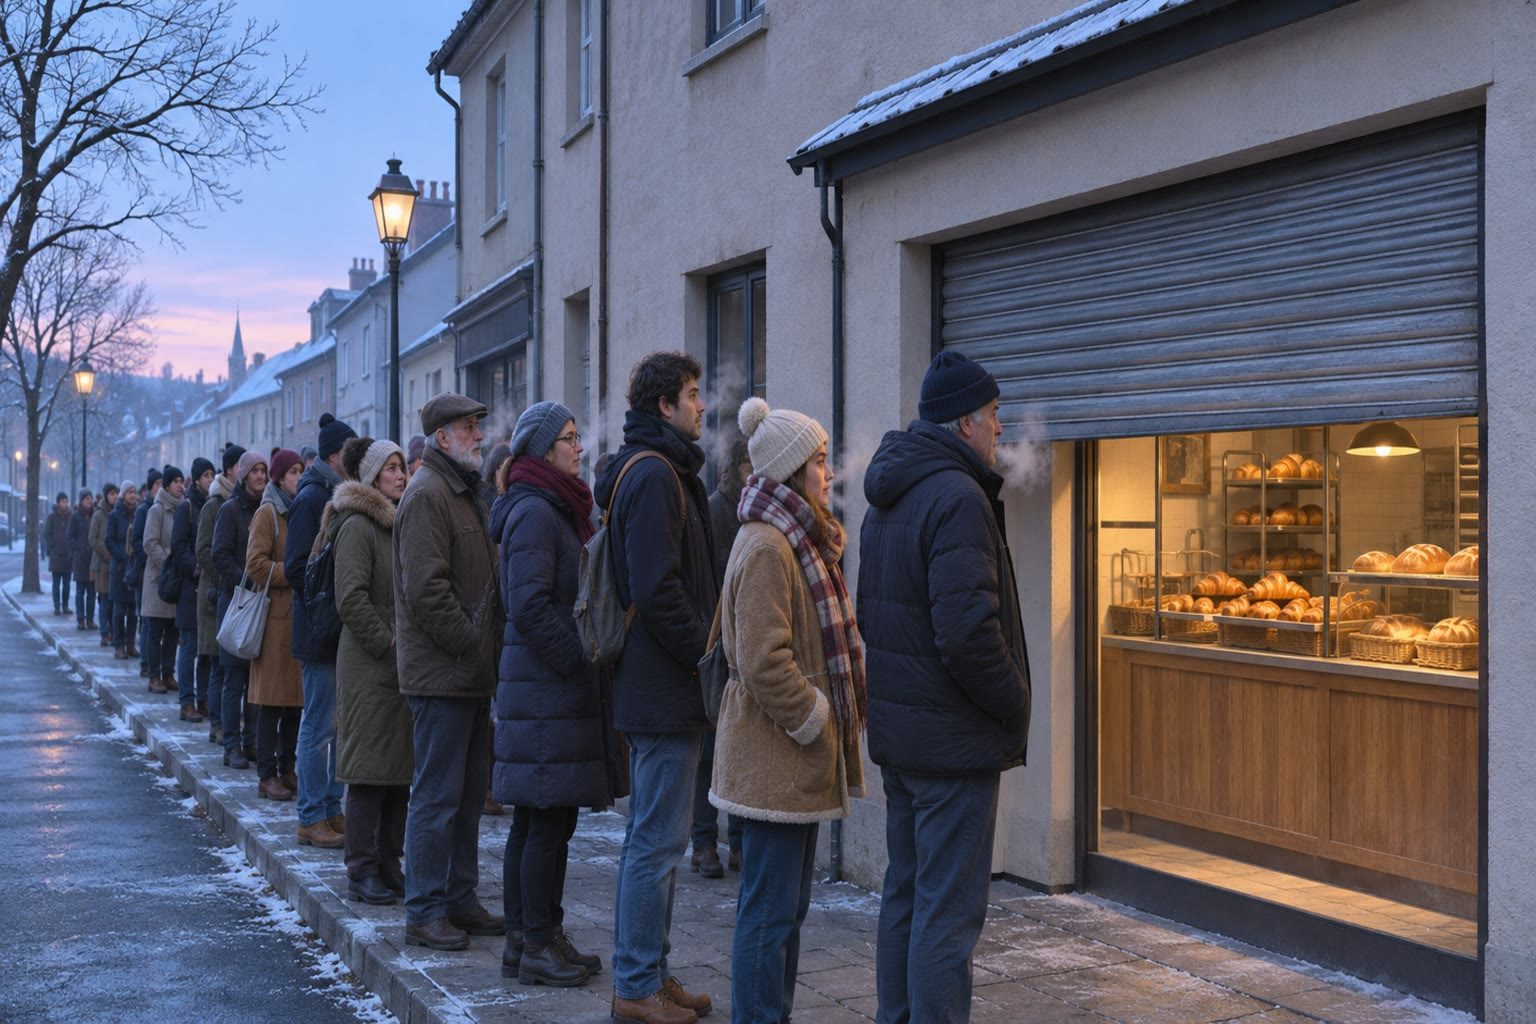
\includegraphics[width=0.5\linewidth]{images/book1/ai/g9-controls-queue-at-dawn.jpg}

{\small A queue outside a bakery before it opens. When a \omterm{def:g7:money:price}{price} cannot rise to match demand, the goods go
to those who come first.}
\end{omfigure}

\section{A minimum price}

\begin{definition}[Price floor]\label{def:g9:price-controls-taxes-subsidies:price-floor}
A \emph{price floor}\index{price floor} is a minimum \omterm{def:g7:money:price}{price} set by law: buyers may not pay less.
\end{definition}

A floor of 12 dalens, above the equilibrium, gives a \omterm{def:g7:demand-and-supply-first-look:quantity-demanded}{quantity demanded} of $120 - 48 = 72$ and a
\omterm{def:g7:demand-and-supply-first-look:quantity-supplied}{quantity supplied} of $20 + 72 = 92$: 20 units are offered and not bought. Governments that set a floor
for a farm product often buy the unsold quantity themselves, and the stock grows year after year.

% figdata: milk (year 1 unsold 100, year 8 unsold 281, stock 1495)
\begin{omchart}{An invented milk market with a floor price: each year the government buys the milk that
is offered and not bought, in millions of litres. Supply grows faster than demand at the floor price, and
the stock keeps growing.}{Invented}
\begin{tikzpicture}
\begin{axis}[omrecord, ybar, bar width=12pt, xmin=0.4, xmax=8.6, ymin=0, ymax=1600, xtick={1,...,8},
  xlabel={Year}, ylabel={Millions of litres}, height=0.42\linewidth, area legend,
  legend style={at={(0.03,0.97)}, anchor=north west}]
\addplot[fill=omDef!45, draw=none, bar shift=0pt] table[x=year, y=stock] {figdata/grade-9/03-price-controls-taxes-subsidies/out/milk.csv};
\addplot[fill=omDef, draw=none, bar shift=0pt, bar width=6pt] table[x=year, y=unsold] {figdata/grade-9/03-price-controls-taxes-subsidies/out/milk.csv};
\legend{stock held by the government, bought this year}
\end{axis}
\end{tikzpicture}
\end{omchart}

\section{A tax per unit}

\begin{definition}[Tax per unit]\label{def:g9:price-controls-taxes-subsidies:tax-per-unit}
A \emph{tax per unit}\index{tax per unit} is a fixed amount of \omterm{def:g7:money:money}{money} paid to the government on each unit
of a good sold.
\end{definition}

Suppose sellers must pay 5 dalens on each unit. When buyers pay a \omterm{def:g7:money:price}{price} $p$, sellers keep $p - 5$, and they
offer what they used to offer at that \omterm{def:g7:money:price}{price}: $Q^s = 20 + 6(p - 5) = -10 + 6p$. The new equilibrium is
\[
120 - 4p = -10 + 6p \quad\Longrightarrow\quad 130 = 10p \quad\Longrightarrow\quad p = 13,
\]
with $120 - 52 = 68$ units sold. Buyers pay 13 dalens, 3 more than before; sellers keep $13 - 5 = 8$
dalens, 2 less than before. The government collects $5 \times 68 = 340$ dalens.

\begin{omchart}{A tax of 5 dalens a unit in the worked example. The supply line, drawn in the price paid
by buyers, moves up by 5 (dashed). Buyers pay 13, sellers keep 8; 68 units are sold instead of
80.}{Invented}
\begin{tikzpicture}
\begin{axis}[omrecord, xmin=0, xmax=160, ymin=0, ymax=20, height=0.5\linewidth,
  xlabel={Quantity (units a day)}, ylabel={Price (dalens)}, xtick={0,40,68,80,120,160},
  ytick={0,5,8,10,13,15,20}]
\addplot[demand] table[x=qd, y=price] {figdata/grade-9/03-price-controls-taxes-subsidies/out/example.csv};
\addplot[supply] table[x=qs, y=price, restrict x to domain=0:160] {figdata/grade-9/03-price-controls-taxes-subsidies/out/example.csv};
\addplot[supply, shifted] table[x=qs_tax, y=price, restrict x to domain=0:160] {figdata/grade-9/03-price-controls-taxes-subsidies/out/example.csv};
\draw[guide] (axis cs:0,13) -- (axis cs:68,13) -- (axis cs:68,0);
\draw[guide] (axis cs:0,8) -- (axis cs:68,8);
\draw[<->, thick] (axis cs:60,8) -- (axis cs:60,13) node[midway, left, font=\scriptsize] {tax 5};
\node[eqpoint] at (axis cs:68,13) {};
\node[eqpoint, fill=black!45] at (axis cs:80,10) {};
\node[anchor=west, font=\footnotesize, text=omDef] at (axis cs:122,1) {demand};
\node[anchor=west, font=\footnotesize, text=omThm] at (axis cs:142,19) {supply};
\node[anchor=east, font=\footnotesize, text=omThm] at (axis cs:100,19) {with the tax};
\end{axis}
\end{tikzpicture}
\end{omchart}

\section{Who bears the tax}

The \omterm{def:g8:taxes-and-public-spending:tax}{tax} is 5 dalens, but buyers pay only 3 more and sellers keep 2 less: the burden is shared. With
$Q^d = a - b\,p$ and $Q^s = c + d\,p$, a \omterm{def:g8:taxes-and-public-spending:tax}{tax} of $t$ per unit raises the buyers' \omterm{def:g7:money:price}{price} by $t \times
d/(b + d)$, and lowers the \omterm{def:g7:money:price}{price} kept by sellers by $t \times b/(b + d)$. Here $d/(b + d) = 6/10$: buyers bear
three fifths of the \omterm{def:g8:taxes-and-public-spending:tax}{tax}. Whoever responds less to the \omterm{def:g7:money:price}{price} bears more of the \omterm{def:g8:taxes-and-public-spending:tax}{tax}: buyers who cannot do
without the good, or sellers who cannot produce less. It makes no difference whether the law says that
buyers or sellers hand the \omterm{def:g8:taxes-and-public-spending:tax}{tax} to the government.

\begin{model}{A tax per unit}
\assumes Many buyers and sellers; a fixed \omterm{def:g8:taxes-and-public-spending:tax}{tax} on each unit sold.
\predicts The \omterm{def:g7:money:price}{price} paid by buyers rises by a part of the \omterm{def:g8:taxes-and-public-spending:tax}{tax} and the \omterm{def:g7:money:price}{price} kept by sellers falls by the
rest; the shares are set by the slopes, $d/(b + d)$ for buyers; fewer units are sold.
\tested When Germany cut its fuel \omterm{def:g8:taxes-and-public-spending:tax}{taxes} for three months from 1 June 2022, the whole cut reached the \omterm{def:g7:money:price}{price}
paid at the pump for gasoline, and at least part of it for diesel (Dovern et al., 2023). In the model, buyers
get the whole change when sellers can offer more at almost the same cost (a very large $d$).
\breaks With few sellers, who may keep part of a \omterm{def:g8:taxes-and-public-spending:tax}{tax} cut or pass on more than a \omterm{def:g8:taxes-and-public-spending:tax}{tax} rise; when the \omterm{def:g8:taxes-and-public-spending:tax}{tax} is
evaded.
\end{model}
% ledger: g9:fuel-tax-cut-2022

\section{A subsidy}

\begin{definition}[Subsidy]\label{def:g9:price-controls-taxes-subsidies:subsidy}
A \emph{subsidy}\index{subsidy} is an amount of \omterm{def:g7:money:money}{money} that a government pays for each unit of a good
produced or sold: a \omterm{def:g8:taxes-and-public-spending:tax}{tax} with a minus sign.
\end{definition}

With a \omterm{def:g9:price-controls-taxes-subsidies:subsidy}{subsidy} of 5 dalens a unit paid to sellers, sellers receive $p + 5$ when buyers pay $p$:
$Q^s = 20 + 6(p + 5) = 50 + 6p$. Then $120 - 4p = 50 + 6p$ gives $p = 7$ and $120 - 28 = 92$ units. Buyers pay
3 dalens less, sellers receive $7 + 5 = 12$, 2 more; the \omterm{def:g9:price-controls-taxes-subsidies:subsidy}{subsidy} costs the government $5 \times 92 = 460$
dalens. Unlike a ceiling, a \omterm{def:g9:price-controls-taxes-subsidies:subsidy}{subsidy} lowers the \omterm{def:g7:money:price}{price} without a \omterm{def:g7:markets-and-prices:shortage}{shortage}, and someone pays for it through
\omterm{def:g8:taxes-and-public-spending:tax}{taxes}.

\begin{record}[A fuel tax cut]
% ledger: g9:fuel-tax-cut-2022
In 2022, Germany lowered its \omterm{def:g8:taxes-and-public-spending:tax}{tax} on fuel for three months, June, July and August.
A study comparing German fuel \omterm{def:g7:money:price}{prices} with those of similar countries without the cut found that for
gasoline the whole \omterm{def:g8:taxes-and-public-spending:tax}{tax} cut was passed on to buyers; for diesel, at least part of it was, and less in
August than in June (Dovern et al., 2023). For gasoline, the \omterm{def:g8:taxes-and-public-spending:tax}{tax} cut worked like a \omterm{def:g9:price-controls-taxes-subsidies:subsidy}{subsidy} of the same
size paid to buyers.
\end{record}

\section{Exercises}

\begin{exercise}[$\star$]\label{exo:g9:price-controls-taxes-subsidies:1}
Use the opening chart. By what percentage did the covered landlords reduce the housing they offered for
rent? What rise in rents across the city do the authors calculate, and how was it obtained?
\end{exercise}

\begin{exercise}[$\star$]\label{exo:g9:price-controls-taxes-subsidies:2}
In the worked example, a ceiling is set at 9 dalens. Compute the \omterm{def:g7:markets-and-prices:shortage}{shortage}.
\end{exercise}

\begin{exercise}[$\star$]\label{exo:g9:price-controls-taxes-subsidies:3}
In the worked example, a floor is set at 11 dalens. Compute the unsold quantity.
\end{exercise}

\begin{exercise}[$\star$]\label{exo:g9:price-controls-taxes-subsidies:4}
With a \omterm{def:g8:taxes-and-public-spending:tax}{tax} of 5 dalens a unit, buyers pay 13 dalens. How much does the seller keep on each unit?
\end{exercise}

\begin{exercise}[$\star\star$]\label{exo:g9:price-controls-taxes-subsidies:5}
In the worked example, the \omterm{def:g8:taxes-and-public-spending:tax}{tax} is 10 dalens a unit. Compute the \omterm{def:g7:money:price}{price} paid by buyers, the \omterm{def:g7:money:price}{price} kept by
sellers, and the quantity sold.
\end{exercise}

\begin{exercise}[$\star\star$]\label{exo:g9:price-controls-taxes-subsidies:6}
Compute the government's \omterm{def:g7:firms:revenue}{revenue} from the \omterm{def:g8:taxes-and-public-spending:tax}{tax} of exercise 5.
\end{exercise}

\begin{exercise}[$\star\star$]\label{exo:g9:price-controls-taxes-subsidies:7}
In the worked example, a ceiling is set at 12 dalens. What happens to the \omterm{def:g7:money:price}{price} and the quantity sold?
\end{exercise}

\begin{exercise}[$\star\star$]\label{exo:g9:price-controls-taxes-subsidies:8}
In the worked example, a \omterm{def:g9:price-controls-taxes-subsidies:subsidy}{subsidy} of 2 dalens a unit is paid to sellers. Compute the \omterm{def:g7:money:price}{price} paid by buyers,
the amount received by sellers, the quantity and the cost of the \omterm{def:g9:price-controls-taxes-subsidies:subsidy}{subsidy}.
\end{exercise}

\begin{exercise}[$\star\star$]\label{exo:g9:price-controls-taxes-subsidies:9}
A town sets a maximum rent, but a year later no flats are missing: anyone who looks for a flat finds one
at the legal rent. Give two possible explanations.
\end{exercise}

\begin{exercise}[$\star\star\star$]\label{exo:g9:price-controls-taxes-subsidies:10}
Demand is $Q^d = 100 - p$ and supply $Q^s = 4p$. Compute the equilibrium, then the \omterm{def:g7:money:price}{prices} paid by buyers
and kept by sellers with a \omterm{def:g8:taxes-and-public-spending:tax}{tax} of 5 dalens a unit. Who bears more of the \omterm{def:g8:taxes-and-public-spending:tax}{tax}?
\end{exercise}

\begin{exercise}[$\star\star\star$]\label{exo:g9:price-controls-taxes-subsidies:11}
Demand is $Q^d = 120 - 4p$. With a \omterm{def:g8:taxes-and-public-spending:tax}{tax} of 5 dalens a unit, by how much does the buyers' \omterm{def:g7:money:price}{price} rise when
supply is $Q^s = 20 + 6p$, and when supply is $Q^s = 70 + p$ (sellers respond little to the \omterm{def:g7:money:price}{price})?
\end{exercise}

\begin{exercise}[$\star\star\star$]\label{exo:g9:price-controls-taxes-subsidies:12}
The study of the opening chart compares the buildings that rent control covered from 1994 with similar
buildings that it did not cover. Why is this better than comparing the covered buildings before and after
1994?
\end{exercise}

\section{Problem: Bread in a Hard Winter}

\begin{problem}[{Weekend problem --- Brenmoor's bread market in winter, a maximum price and its shortage,
and a subsidy per loaf instead}]
\label{pb:g9:price-controls-taxes-subsidies:1}
Everything in this problem is invented. In a hard winter, flour becomes dear. Brenmoor's bakers offer
$Q^s = -2\,000 + 2\,000\,p$ loaves a day at a \omterm{def:g7:money:price}{price} of $p$ dalens, and the town's families want
$Q^d = 7\,000 - 1\,000\,p$ loaves.

\medskip
\noindent\textbf{Part I --- The market.}
\begin{enumerate}
  \item Compute the \omterm{def:g7:demand-and-supply-first-look:quantity-demanded}{quantity demanded} at 2 and at 3 dalens.
  \item Compute the \omterm{def:g7:demand-and-supply-first-look:quantity-supplied}{quantity supplied} at 2 and at 3 dalens.
  \item Find the \omterm{def:g7:demand-and-supply-first-look:equilibrium-price}{equilibrium price} and quantity.
  \item Compute the bakers' daily \omterm{def:g7:firms:revenue}{revenue} at the equilibrium.
\end{enumerate}

\medskip
\noindent\textbf{Part II --- A maximum price.} The town sets a maximum \omterm{def:g7:money:price}{price} of $2.50$ dalens a loaf.
\begin{enumerate}[resume]
  \item Compute the quantities demanded and supplied, and the \omterm{def:g7:markets-and-prices:shortage}{shortage}.
  \item How many loaves are sold each day?
  \item At what \omterm{def:g7:money:price}{price} would families want only the loaves that are sold? (This is about the \omterm{def:g7:money:price}{price} a
        black \omterm{def:g7:markets-and-prices:market}{market} could reach.)
  \item Name two other things that may happen while the maximum \omterm{def:g7:money:price}{price} lasts.
\end{enumerate}

\medskip
\noindent\textbf{Part III --- A subsidy instead.} The town removes the maximum \omterm{def:g7:money:price}{price} and pays bakers a
\omterm{def:g9:price-controls-taxes-subsidies:subsidy}{subsidy} per loaf, so that families pay $2.50$ dalens and no loaf is missing.
\begin{enumerate}[resume]
  \item How many loaves do families want at $2.50$ dalens?
  \item What \omterm{def:g7:money:price}{price} must bakers receive to offer that many loaves?
  \item What \omterm{def:g9:price-controls-taxes-subsidies:subsidy}{subsidy} per loaf is needed?
  \item What does the \omterm{def:g9:price-controls-taxes-subsidies:subsidy}{subsidy} cost the town each day?
  \item Compare with Part I: the \omterm{def:g7:money:price}{price} paid by families, the amount received by bakers, the number of
        loaves. Who pays for the difference?
\end{enumerate}
\end{problem}
